
\begin{frame}
		\frametitle{Parallel Sort}
		\begin{figure}
				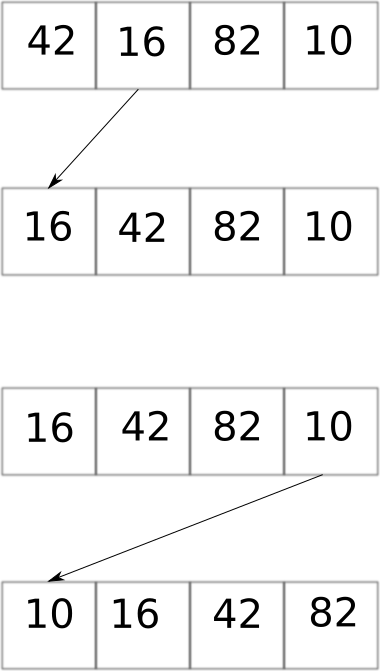
\includegraphics[width=0.3\linewidth]{figures/diagrams/sort/serialsort}
		\end{figure}	
\end{frame}

\begin{frame}
		\frametitle{Parallel Sort}
		\begin{figure}
				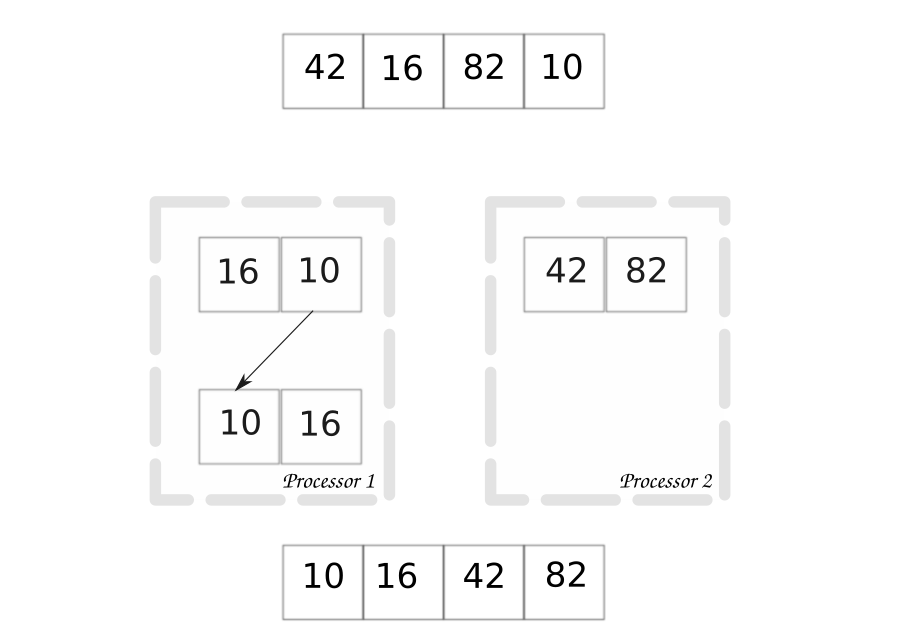
\includegraphics[width=0.8\linewidth]{figures/diagrams/sort/parallelsort}
		\end{figure}	
\end{frame}

\begin{frame}
		\frametitle{Parallel CLI}
		abyss-pe np=8\newline
		bowtie2 -p 8\newline
		namd +p 12 +ppn 3\newline
		sort --parallel=8\newline
\end{frame}


\begin{frame}[fragile]
		\frametitle{Parallel Code}
		\begin{verbatim}
			library(doParallel)
			cl <- makeCluster(2)
			registerDoParallel(cl)
			foreach(i=1:3) %dopar% sqrt(i)
		\end{verbatim}
\end{frame}

\begin{frame}
		\frametitle{Observed Speedup}
		\begin{figure}
				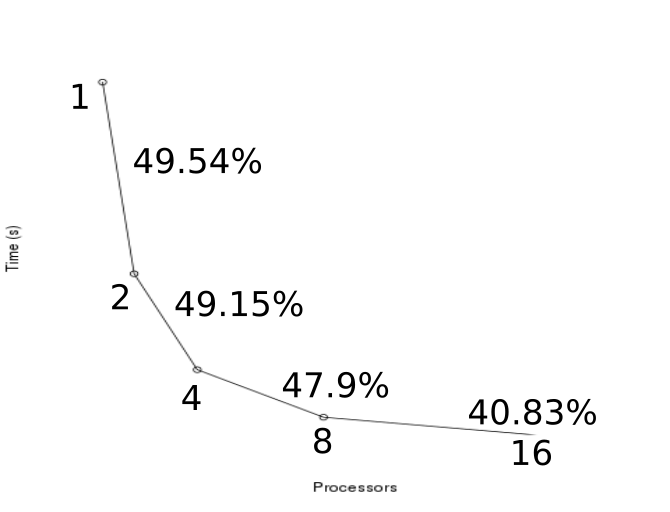
\includegraphics[width=0.7\linewidth]{figures/diagrams/omp/reduction}
		\end{figure}
\end{frame}

\begin{frame}
		\frametitle{Observed Speedup}
		We observed 92\% speedup.
\end{frame}


\begin{frame}
		\frametitle{Amdahl's law}
		\begin{figure}
				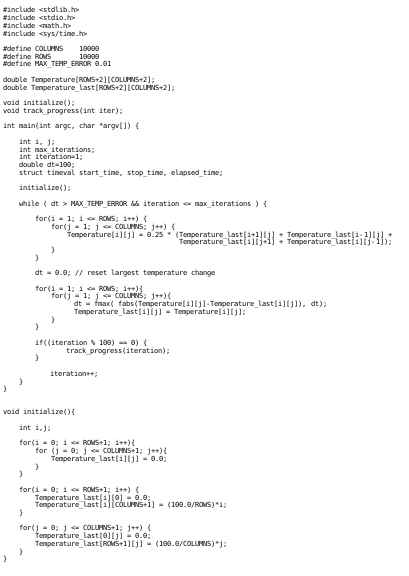
\includegraphics[width=0.4\linewidth]{figures/diagrams/amdahl/code}
		\end{figure}
\end{frame}

\begin{frame}
		\frametitle{Amdahl's law}
		\begin{figure}
				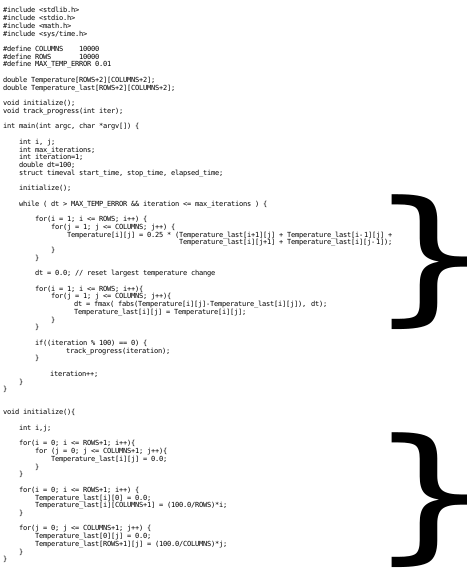
\includegraphics[width=0.4\linewidth]{figures/diagrams/amdahl/parallelblocks}
		\end{figure}
\end{frame}

\begin{frame}
		\frametitle{Amdahl's law}
		72 total lines of code 

		24 parallelizable lines of code


		\color{red}Parallel computing will only reduce time spent computing
		34\% of the total application.
\end{frame}

\begin{frame}
		\frametitle{Parallel Overhead}
		\begin{figure}
				\includegraphics[width=0.4\linewidth]{figures/diagrams/amdahl/overhead}
		\end{figure}
\end{frame}

\begin{frame}
		\frametitle{Parallel Overhead}
		\sout{Reduce time spent on 34\% of application!}\newline

		\color{red}Due to parallelization overhead, theorectical limit isn't
even possible.
\end{frame}

